\chapter{Определения}
\label{chap:surfaces-def}

\section{Топологические поверхности}

В основном нас будут интересовать гладкие поверхности, определённые в следующем разделе.
Сейчас мы дадим более общее определение, которое будет использоваться лишь пару раз.

Связное подмножество $\Sigma$ евклидова пространства $\mathbb{R}^3$
называется \index{поверхность}\index{топологическая!поверхность}\emph{топологической поверхностью} (точнее {}\emph{вложенной топологической поверхностью без границы}),
если любая точка $p\in \Sigma$ имеет окрестность $W$ в $\Sigma$,
которую можно параметризовать открытым подмножеством евклидовой плоскости;
то есть существует гомеоморфизм $U\to W$ из открытого множества $U\subset \mathbb{R}^2$; см.~\ref{sec:topology}.

\section{Гладкие поверхности}\label{sec:def-smooth-surface}

Напомним, что функция $f$ двух переменных $x$ и $y$ называется \index{гладкая!функция}\emph{гладкой}, если все её частные производные $\frac{\partial^{m+n}}{\partial x^m\partial y^n}f$ определены (а значит, и непрерывны) в области определения~$f$.

{\sloppy

Связное множество $\Sigma \subset \mathbb{R}^3$ называется \index{поверхность}\index{гладкая!поверхность}\emph{гладкой поверхностью}%
\footnote{Это сокращение термина {}\emph{гладкая регулярная вложенная поверхность}.}, если оно локально описывается как график гладкой функции в подходящей системе координат.

Точнее, для любой точки $p\in \Sigma$ найдётся система координат $(x,y,z)$ и окрестность $U\ni p$ так, что
пересечение $W=U\cap \Sigma$ задаётся графиком $z=f(x,y)$ гладкой функции $f$, определённой в открытой области плоскости $(x,y)$.

}

\parbf{Примеры.}
Координатная плоскость
$\Pi=\set{(x,y,z)\in\mathbb{R}^3}{z=0}$
даёт пример гладкой поверхности, ведь она является графиком функции $f(x,y)=0$.

Любая другая плоскость также являются гладкой поверхностью, ведь она координатная в подходящей системе координат.
Можно также представить плоскость как график линейной функции 
$f(x,y)\z=a\cdot x+b\cdot y+c$ для некоторых констант $a$, $b$ и $c$
(предполагая, что плоскость не вертикальна, иначе придётся взять другие координаты).

Более хитрый пример даёт единичная сфера 
\[\mathbb{S}^2=\set{(x,y,z)\in\mathbb{R}^3}{x^2+y^2+z^2=1}.\]
Вся сфера не является графиком,
однако её можно покрыть 6 графиками:
\begin{align*}
z&=f_\pm(x,y)=\pm \sqrt{1-x^2-y^2},
\\
y&=g_\pm(x,z)=\pm \sqrt{1-x^2-z^2},
\\
x&=h_\pm(y,z)=\pm \sqrt{1-y^2-z^2},
\end{align*}
где каждая функция $f_+$, $f_-$, $g_+$, $g_-$, $h_+$ и $h_-$ определена в открытом единичном круге.
Любая точка $p\in\mathbb{S}^2$ лежит на одном из этих графиков, следовательно, $\mathbb{S}^2$ --- гладкая  поверхность.

\section{Поверхности с краем}

{\sloppy

Связное подмножество поверхности, ограниченное одной или несколькими кусочно гладкими кривыми, называется \index{поверхность!с краем}\emph{поверхностью с краем}; эти кривые и образуют \index{край}\emph{край} поверхности.

}

Как правило, мы говорим {}\emph{поверхность}, имея в виду {}\emph{гладкую поверхность без края}.
При необходимости, можно использовать термин {}\emph{поверхность с возможно непустым краем}.


\section{Типы поверхностей}

Если поверхность $\Sigma$ образует замкнутое множество в $\mathbb{R}^3$, то она называется \index{собственная!поверхность}\emph{собственной}.
Например, график $z=f(x,y)$ любой гладкой функции $f$, определённой на всей плоскости, является собственной поверхностью.
Сфера $\mathbb{S}^2$ --- другой пример собственной поверхности.

С другой стороны, открытый круг 
\[\set{(x,y,z)\in\mathbb{R}^3}{x^2+y^2<1,\  z=0}\]
не собственная поверхность; он не открыт, и не замкнут в $\mathbb{R}^3$.

{\sloppy

Компактная поверхность без края называется \index{замкнутая!поверхность}\emph{замкнутой}
(по аналогии с замкнутой кривой, но без связи с замкнутым множеством).

}

\index{открытая!поверхность}\emph{Открытая} поверхность --- это
собственная некомпактная поверхность без края 
(опять же, термин связан с открытой кривой, но не с открытым множеством).

Для примера, параболоид $z=x^2+y^2$ --- открытая поверхность,
а сфера $\mathbb{S}^2$ --- замкнутая.
Заметим, что \textit{любая собственная поверхность без края замкнута или открыта}.

Следующее факт является трёхмерным аналогом теоремы Жордана (\ref{ex:proper-curve}).
Оно вовсе не очевидно.
Доказательство использует так называемую {}\emph{двойственность Александера} \cite{hatcher}, но мы его опускаем.
Оно бы увело нас далеко в сторону.

\begin{thm}{Факт}\label{clm:proper-divides}
Дополнение любой собственной топологической поверхности без края (эквивалентно, любой открытой или замкнутой топологической поверхности) имеет ровно две связные компоненты.
\end{thm}


\section{Неявно заданные поверхности}

\begin{thm}{Предложение}\label{prop:implicit-surface}
Предположим, что $0$ --- регулярное значение гладкой функции $f\:\mathbb{R}^3\to \mathbb{R}$;
то есть $\nabla_p f\ne 0$ если $f(p)=0$.
Тогда любая компонента связности $\Sigma$ множества уровня $f(x,y,z)=0$ является гладкой поверхностью.
\end{thm}

\parbf{Доказательство.}
Выберем точку $p\in\Sigma$.
Так как $\nabla_p f\ne 0$, выполнятся какое-то из условий 
$f_x(p)\ne 0$,
$f_y(p)\ne 0$ или
$f_z(p)\ne 0$.
Можно предположить, что $f_z(p)\ne 0$;
иначе, переименуем координаты $x,y,z$.

По теореме о неявной функции (\ref{thm:imlicit}), окрестность $p$ в $\Sigma$ является графиком $z=h(x,y)$ гладкой функции $h$, определённой на открытом множестве в $\mathbb{R}^2$.
Остаётся применить определение гладкой поверхности (см.~\ref{sec:def-smooth-surface}).
\qeds

\begin{thm}{Упражнение}\label{ex:hyperboloids}
При каких $\ell$ множество уровня $x^2+y^2-z^2=\ell$ является гладкой поверхностью?
\end{thm}

\section{Локальные параметризации}
\index{параметризация}

Пусть $U$ --- открытая область в $\mathbb{R}^2$, и $s\:U\to \mathbb{R}^3$ --- гладкое отображение;
оно называется \index{регулярная!параметризация}\emph{регулярным} если его матрица Якоби имеет максимальный ранг в любой точке.
В данном случае это означает, что производные $s_u$ и $s_v$ линейно независимы в любой точке $(u,v)\in U$;
эквивалентно $s_u\times s_v\ne 0$, где $\times$ обозначает векторное произведение.

\begin{thm}{Предложение}\label{prop:graph-chart}
Образ $\Sigma=s(U)$ гладкого регулярного вложения $s$ открытого связного множества $U\subset \mathbb{R}^2$ является гладкой поверхностью.
\end{thm}

\parbf{Доказательство \ref{prop:graph-chart}.}
Пусть $s(u,v)=(x(u,v),y(u,v),z(u,v))$.
Поскольку $s$ регулярно, матрица Якоби
\[\Jac s=
\renewcommand\arraystretch{1.3}
\begin{pmatrix}
x_u&x_v\\
y_u&y_v\\
z_u&z_v
\end{pmatrix}
\]
имеет ранг два в любой точке $(u,v)\in U$.

Выберем точку $p\in \Sigma$; сдвинув координаты $(x,y,z)$ и $(u,v)$, можно считать, что $p = (0,0, 0) =s(0,0)$.
Переименовав координаты $x,y,z$, можно добиться чтобы 
матрица $\left(\begin{smallmatrix}
x_u&x_v\\
y_u&y_v
\end{smallmatrix}\right)$
стала обратима в начале координат.
Отметим, что это матрица Якоби для $(u,v)\mapsto (x(u,v),y(u,v))$.

По теореме об обратной функции (\ref{thm:inverse}), существует гладкое регулярное отображение
$w\:(x,y)\mapsto (u,v)$, определённое на открытом множестве $W\ni 0$ в плоскости $(x,y)$,
 что $w(0,0)=(0,0)$ и $s\circ w(x,y)=(x,y,f(x,y))$, где $f=z\circ w$.
То есть, подмножество $s\circ w(W)\subset \Sigma$ является графиком $f$.

И снова по теореме об обратной функции, образ $w(W)$ открыт в $U$.
Поскольку $s$ --- вложение, наш график открыт в~$\Sigma$;
то есть существует такое открытое множество $V\subset \mathbb{R}^3$, что $s\circ w(W)=V\cap \Sigma$ --- график гладкой функции.
А это уже означает, что $\Sigma$ гладкая поверхность, ведь $p$ выбиралась произвольно.
\qeds


\begin{thm}{Упражнение}\label{ex:9-surf}
Найдите гладкое регулярное инъективное отображение $s\:\mathbb{R}^2\to\mathbb{R}^3$ образ которого \textit{не} является поверхностью.
\end{thm}

Если $s$ и $\Sigma$, как в предложении, то $s$ называется \index{гладкая!параметризация}\emph{гладкой параметризацией} поверхности~$\Sigma$. 

Не все гладкие поверхности можно так запараметризовать;
например, сферу $\mathbb{S}^2$ нельзя.
Однако, \textit{любая гладкая поверхность $\Sigma$ допускает локальную параметризацию в любой точке $p\in\Sigma$}; то есть $p$ имеет открытую окрестность $W\subset \Sigma$ с гладкой регулярной параметризацией~$s$.
В этом случае любая точка в $W$ может быть описана двумя параметрами, обычно обозначаемыми как $u$ и $v$;
они называются \index{локальные координаты}\emph{локальными координатами} при~$p$.
Отображение $s$ называется \index{карта}\emph{картой} поверхности~$\Sigma$.

Если $W$ --- график $z=h(x,y)$ гладкой функции $h$, то отображение 
\[s\:(u,v)\mapsto (u,v,h(u,v))\] является картой.
Действительно, отображение $(u,v,h(u,v))\mapsto (u,v)$ является обратным к $s$, и оно непрерывно;
то есть $s$ --- вложение.
Кроме того,
$s_u\z=(1,0,h_u)$ и $s_v\z=(0,1,h_v)$. 
В частности, $s_u$ и $s_v$ линейно независимы;
то есть $s$ регулярно.

\begin{thm}{Следствие}\label{cor:reg-parmeterization}
Связное множество $\Sigma\subset \mathbb{R}^3$ является гладкой поверхностью тогда и только тогда, когда у любой точки в $\Sigma$ есть 
окрестность в $\Sigma$, которую можно покрыть картой.
\end{thm}

Функция $g\: \Sigma \to \mathbb{R}$, определённая на гладкой поверхности $\Sigma$, называется \index{гладкая!функция}\emph{гладкой}, если для любой карты $s \: U\to \Sigma$,
композиция $g\circ s$ гладкая; то есть все частные производные $\frac{\partial^{m+n}}{\partial u^m\partial v^n}(g\circ s)$ определены и непрерывны в области определения.


\begin{thm}{Упражнение}\label{ex:smooth-fun(surf)}
Пусть $\Sigma\subset \mathbb{R}^3$ --- гладкая поверхность.
Покажите, что функция $g\:\Sigma\to\mathbb{R}$ --- гладкая тогда и только тогда, когда для любой точки $p\in \Sigma$ существует гладкая функция $h\:N\to\mathbb{R}$, определённая в окрестности $N\subset \mathbb{R}^3$ точки $p$ такая, что равенство $g(q)=h(q)$ выполняется для $q\in \Sigma\cap N$.

Постройте гладкую поверхность $\Sigma$ с гладкой функцией $g\:\Sigma\to\mathbb{R}$, которую невозможно продолжить до гладкой функции $h\:\mathbb{R}^3\to\mathbb{R}$.
\end{thm}

\begin{thm}{Упражнение}\label{ex:inversion-chart}
Покажите, что
\[s(u,v)=(\tfrac{2\cdot u}{1+u^2+v^2},\tfrac{2\cdot v}{1+u^2+v^2},\tfrac{2}{1+u^2+v^2}).\]
является картой единичной сферы с центром в точке $(0,0,1)$; опишите образ~$s$.
\end{thm}

\begin{wrapfigure}{r}{31 mm}
\vskip-6mm
\centering
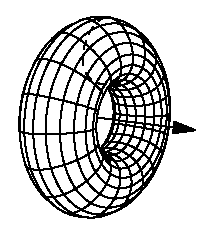
\includegraphics{asy/torus}
\vskip0mm
\end{wrapfigure}

Пусть $\gamma(t)=(x(t),y(t))$ --- кривая на плоскости.
Напомним, что \index{поверхность!вращения}\emph{поверхность вращения} кривой $\gamma$ вокруг оси $x$ описывается как образ отображения 
\[(t, s)\mapsto (x(t), y(t)\cdot\cos s,y(t)\cdot\sin s).\]
При этом параметры $t$ и $s$ называются соответственно \index{широта}\emph{широтой} и \index{долгота}\emph{долготой};
для фиксированных $t$ или $s$ полученные кривые называются \index{параллель}\emph{параллелями} или
\index{меридиан}\emph{меридианами} соответственно. 
Отметим, что параллели образованы окружностями в плоскости, перпендикулярной оси вращения.
Кривая $\gamma$ называется \index{образующая}\emph{образующей} этой поверхности.

\begin{thm}{Упражнение}\label{ex:revolution}
Предположим, что $\gamma$ --- простая замкнутая гладкая плоская кривая, которая не пересекает ось $x$.
Покажите, что поверхность вращения вокруг оси $x$ с образующей $\gamma$ является гладкой поверхностью.
\end{thm}

\section{Глобальные параметризации}\label{sec:global-parametrizations}
\index{параметризация}

Поверхность можно описать как вложение другой поверхности.

Для примера, рассмотрим эллипсоид
\[\Theta=\set{(x,y,z)\in\mathbb{R}^3}{\tfrac{x^2}{a^2}+\tfrac{y^2}{b^2}+\tfrac{z^2}{c^2}=1},\]
где $a$, $b$ и~$c$ --- положительные константы.
По \ref{prop:implicit-surface}, $\Theta$ --- гладкая поверхность.
Действительно, пусть $h(x,y,z)\df\tfrac{x^2}{a^2}+\tfrac{y^2}{b^2}+\tfrac{z^2}{c^2}$,
тогда
\[\nabla h(x,y,z)=(\tfrac{2}{a^2}\cdot x,\tfrac{2}{b^2}\cdot y,\tfrac{2}{c^2}\cdot z).\]
Следовательно, $\nabla h\ne0$, если $h=1$; то есть $1$ является регулярным значением~$h$.
Остаётся заметить, что множество $\Theta$ связно.

Поверхность $\Theta$ задаётся как образ сферы $\mathbb{S}^2$ при отображении
\[(x,y,z)\z\mapsto (a\cdot x, b\cdot y,c\cdot z).\]

Отображение $f\:\Sigma \to \mathbb{R}^3$ (или $f\:\Sigma \to \mathbb{R}^2$) считается гладким, если гладкие все его координатные функции.
Кроме того, гладкое отображение $f \: \Sigma \to \mathbb{R}^3$ называется 
\emph{гладкой параметризованной поверхностью}, если оно является вложением, и для любой карты $s \:U\to \Sigma$,
композиция $f\circ s$ регулярна;
то есть два вектора 
$\frac{\partial}{\partial u}(f\circ s)$ и $\frac{\partial}{\partial v}(f\circ s)$ являются линейно независимыми.
В этом случае, образ $\Sigma^{*}=f(\Sigma)$ --- гладкая поверхность, ведь для любой карты $s\:U\to \Sigma$ композиция $f\circ s\:U\to \Sigma^{*}$ задаёт карту на $\Sigma^{*}$. 

Такое отображение $f$ называется \index{диффеоморфизм}\emph{диффеоморфизмом} из $\Sigma$ в $\Sigma^{*}$;
говорят, что поверхности $\Sigma$ и $\Sigma^{*}$ {}\emph{диффеоморфны}, если существует диффеоморфизм $f\:\Sigma\to\Sigma^{*}$.
Следующее упражнение говорит, что \textit{быть диффеоморфными} --- это отношением эквивалентности.

\begin{thm}{Упражнение}\label{ex:inv-diffeomorphism}
Докажите, что обратное отображение к диффеоморфизму также диффеоморфизм.
\end{thm}

\begin{thm}{Продвинутое упражнение}\label{ex:star-shaped-disc}
Докажите, следующее:

\begin{subthm}{ex:plane-n}
Дополнения $n$-точечных подмножеств плоскости диффеоморфны между собой.
\end{subthm}

\begin{subthm}{ex:star-shaped-disc:smooth}
Открытые выпуклые множества плоскости ограниченные замкнутыми гладкими кривыми диффеоморфны между собой.
\end{subthm}

{\sloppy

\begin{subthm}{ex:star-shaped-disc:nonsmooth}
Любые открытые выпуклые множества плоскости диффеоморфны между собой.
\end{subthm}

\begin{subthm}{ex:star-shaped-disc:star-shaped}
Любые открытые звёздные множества плоскости диффеоморфны между собой.
\end{subthm}

}

\end{thm}
